\chapter{Web Projects}


    \FloatBarrier
    \section{Installing tools}
    
In order to obtain the essential tools for creating website projects with Visual Studio, we have to open the Visual Studio Installer as an administrator and click on \textit{Modify}. We must select in the \textit{Workloads} (in the tab reserved for Web and Cloud) the tools related to ``ASP.NET and web'' with the predefined optional installations selected (see Figure \ref{fig:pro1}). After that, we click on \textit{Modify} and wait for the process to finish the download and installation.

\begin{figure}
    \centering
    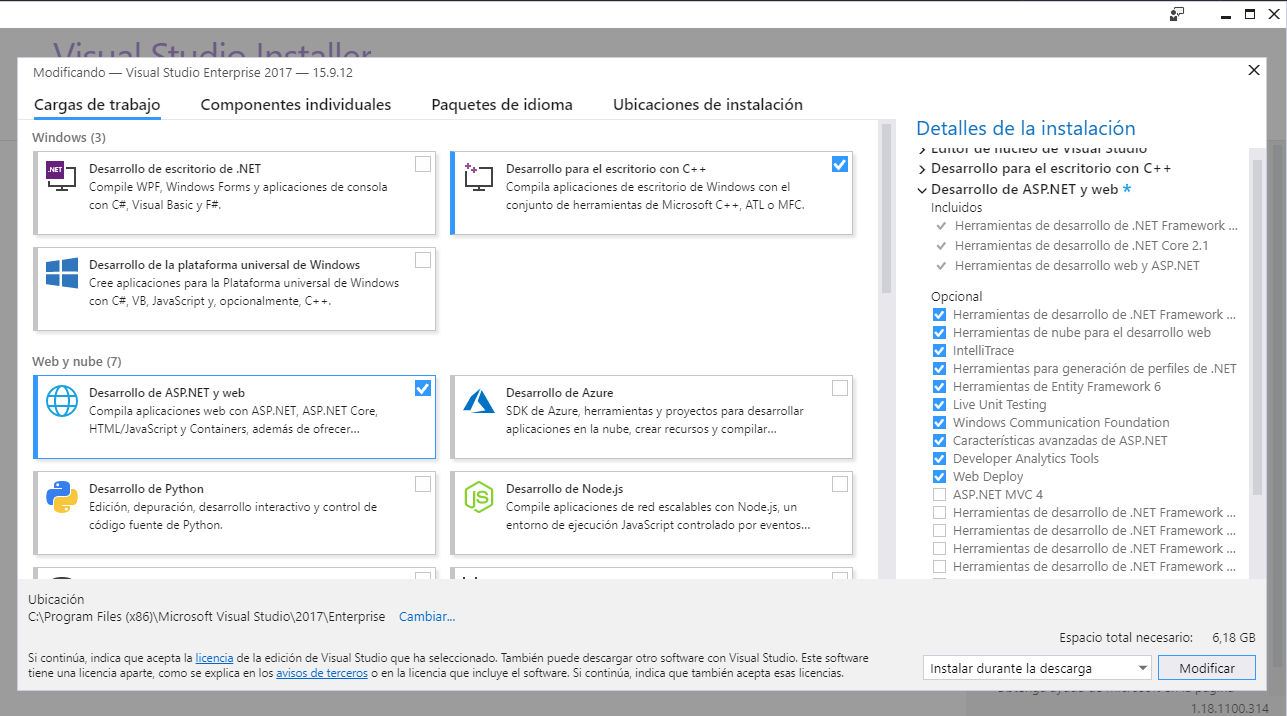
\includegraphics[width= \textwidth]{Figures/Projects/pro1}
    \caption{Main window of Visual Studio Installer with the Workload related to the web programming tools selected.}
    \label{fig:pro1}
\end{figure}




    \FloatBarrier
    \section{Create Website HTML/CSS/JS project}
    
In this section the basic tools for creating web projects with Visual Studio are treated (HTML/CSS/JS). First of all, we have to open Visual Studio and create a solution with a similar template to the one we want, an ``ASP.NET Empty Web Site''. 

\begin{enumerate}
    \item Open your version of Visual Studio.
    \item Go to \textit{FILE/New/Project...}.
    \item In the tab \textit{Installed/Visual C\#/Web/Previous Versions} click on 
    
    \textit{ASP.NET Empty Web Site} (see Figure \ref{fig:pro2}).
    
    \item Choose a name for the project. For example choose ``myWebSite''.
    \item Change the \textit{Location} of the solution, a directory will be created there. In this case it is stored in the Desktop but choose the right location for yours.
    \item Choose the name of the solution (``myWebSiteSolution'' for example), it does not have to be the same as the name of the project. 
    \item Select the option \textit{Create directory for solution}.
    \item Click on \textit{OK}.
\end{enumerate}

\begin{figure}
    \centering
    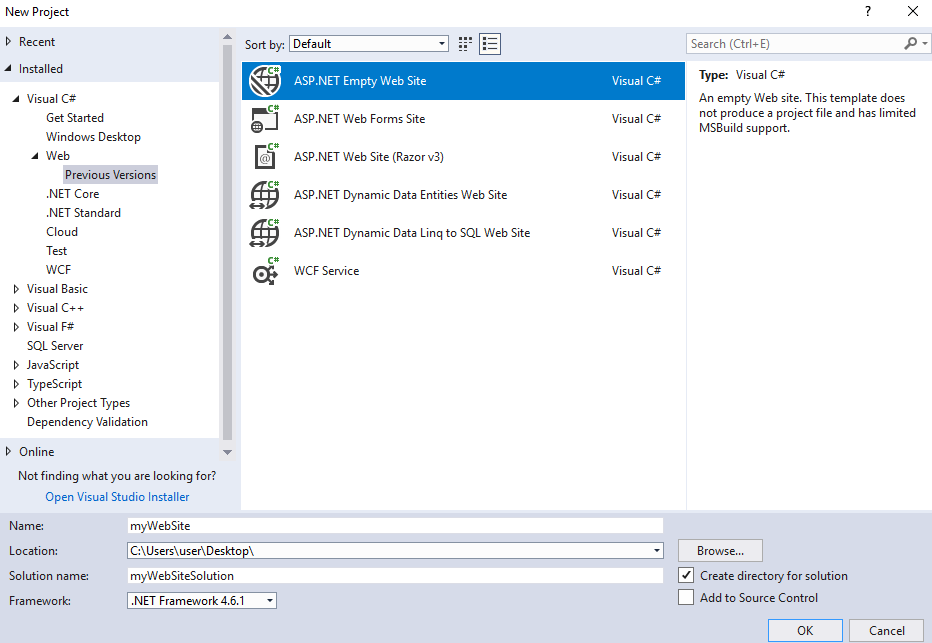
\includegraphics[width= 0.9 \textwidth]{Figures/Projects/pro2}
    \caption{``New Project'' window of Visual Studio with the project template selected, the name of both the project and the solution are already written.}
    \label{fig:pro2}
\end{figure}

The project is created with the default files and folders (see Figure \ref{fig:pro3}) but we prefer to use the structure explained in this guide: \texttt{index.html}, CSS folder, JS folder and images folder if needed:

\begin{enumerate}
    \item Firstly, click with the right button on the name of the project (in the Solution Explorer/myWebSite) and go to \textit{Add/Add New Item...}.
    \item In the tab \textit{Installed/Visual C\#} click on \textit{HTML Page} and call it ``index.html'' (see Figure \ref{fig:pro4a}).
    \item Then, click on \textit{Add} and a basic template will be created in your project (Figure \ref{fig:pro4b}).
\end{enumerate}

\begin{figure}
    \centering
    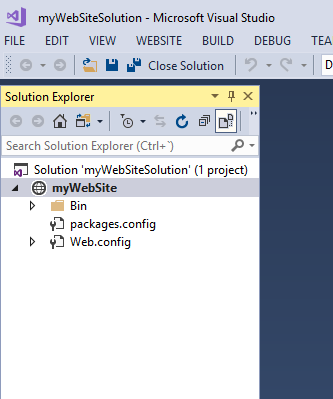
\includegraphics[width= 0.5 \textwidth]{Figures/Projects/pro3}
    \caption{Initial aspect of the Solution and Project created for the Website.}
    \label{fig:pro3}
\end{figure}

\begin{figure}
    \centering
    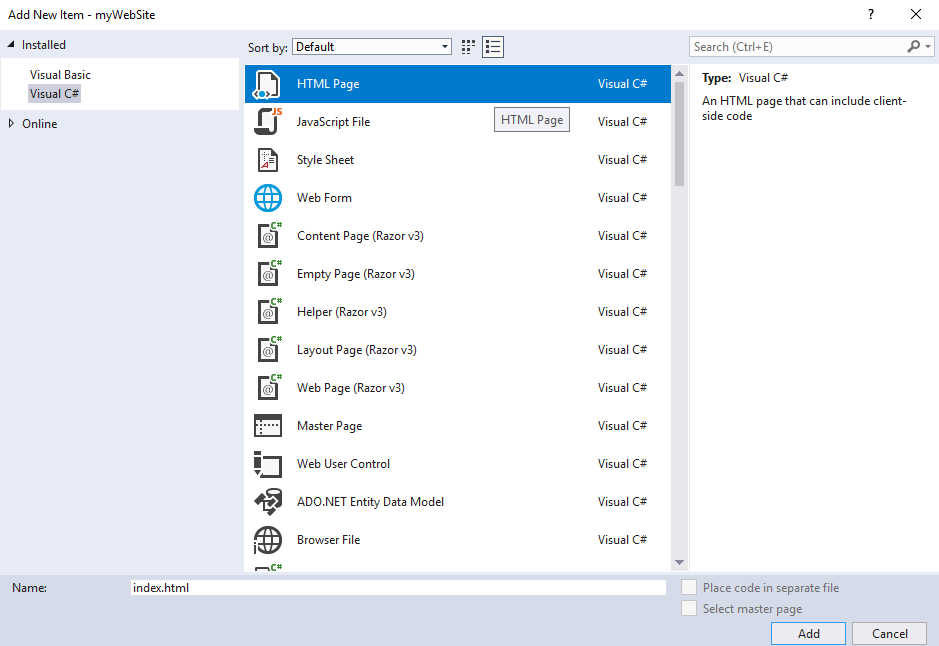
\includegraphics[width= \textwidth]{Figures/Projects/pro4a}
    \caption{Adding \texttt{index.html} to our website using the \textit{Add New Item} window of Visual Studio.}
    \label{fig:pro4a}
\end{figure}

\begin{figure}
    \centering
    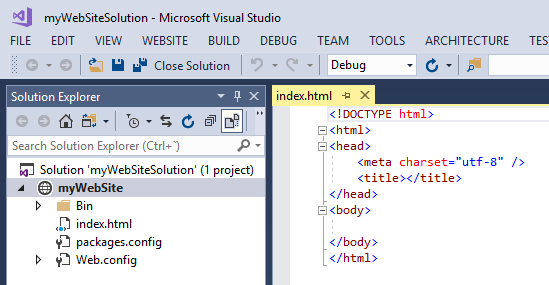
\includegraphics[width= 0.9 \textwidth]{Figures/Projects/pro4b}
    \caption{Template of the \texttt{index.html} file (created by default), here the website is going to be built.}
    \label{fig:pro4b}
\end{figure}

\newpage
Now we are going to create the desired folder structure, right click on the name of the project once again and go to \textit{Add/New Folder}, give it the name ``css''. Repeat the process twice with the names ``js'' and ``img'', the final aspect of your project should be like the seen in Figure \ref{fig:pro5}.

\begin{figure}
    \centering
    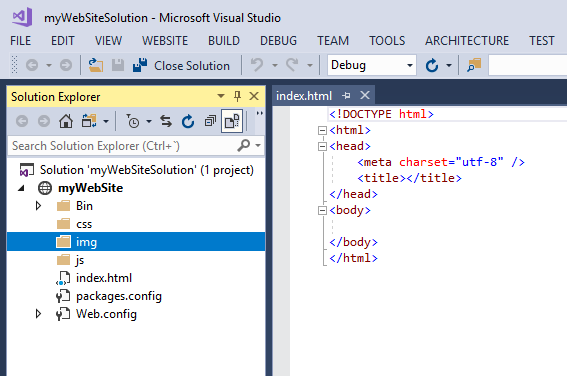
\includegraphics[width= 0.8 \textwidth]{Figures/Projects/pro5}
    \caption{Final folder structure of the project, the files ``css'', ``js'' and ``img'' are not included by default.}
    \label{fig:pro5}
\end{figure}




    \FloatBarrier
    \section{Execute the ``Hello world'' example} \label{sec:Web}

%-----------------------------------------------------------------------------------------------------------------------------    
Now we are going to ``write'' our website starting by a simple example. \textbf{In the first step}, we have to make our initial \texttt{index.html} template looks like the Figure \ref{fig:pro6}. Do not forget to save the changes each time you make a modification in the webpage. 

\begin{figure}
    \centering
    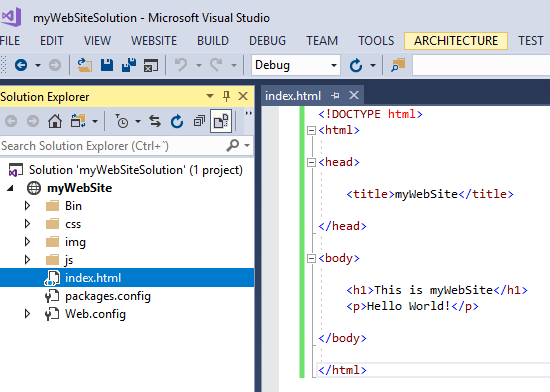
\includegraphics[width= 0.9 \textwidth]{Figures/Projects/pro6}
    \caption{First example of website, the \texttt{index.html} file has been modified.}
    \label{fig:pro6}
\end{figure}

If we want to open our website we can go to the location of the project, open the folder ``myWebSite'' and double click on our \texttt{index.html} file (or just drag it into our browser: Chrome or Firefox for example). However, we want to use Visual Studio for this project so we are going to Build and Start our website using the IDE. 

The Figure \ref{fig:pro7} shows the toolbar \textit{Build} where the Build and Start commands are. We have to click first on \textit{Build} and later in \textit{Start} and Visual Studio will automatically show the output. In addition, a Chrome window (or the default browser) will be opened with our result. If we do not have the mentioned toolbar shown in the environment (highly recommended) we can also click on \textit{BUILD/Build Web Site} and later on \textit{DEBUG/Start without Debugging}. The result of our webpage is shown in the Figure \ref{fig:pro8}.

\begin{figure}
    \centering
    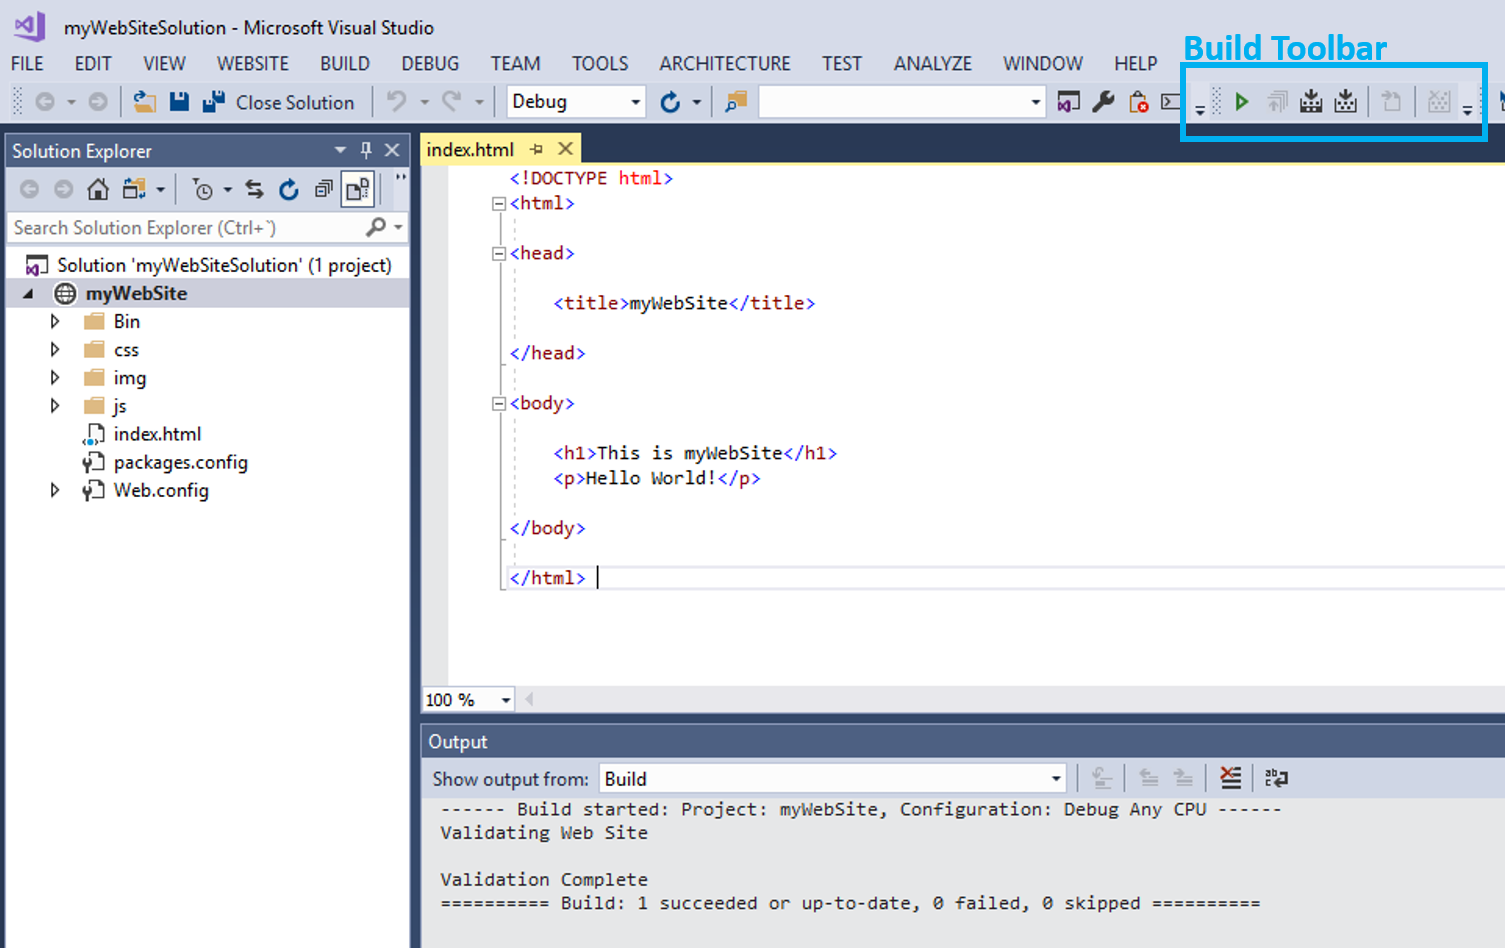
\includegraphics[width= 0.9 \textwidth]{Figures/Projects/pro7}
    \caption{The window Output shows results of the execution. The \textit{Build} toolbar appears remarked in the upper part of the IDE.}
    \label{fig:pro7}
\end{figure}

\begin{figure}
    \centering
    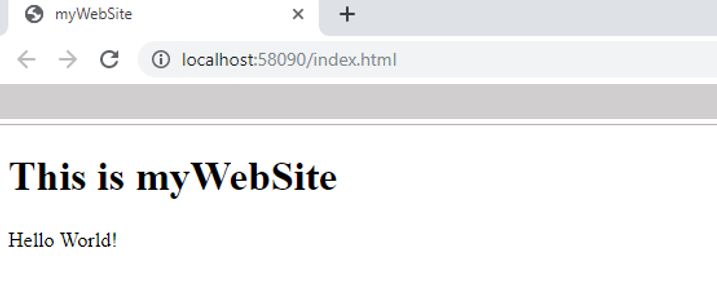
\includegraphics[width= 0.9 \textwidth]{Figures/Projects/pro8}
    \caption{Result of ``myWebSite'' project presented in Google Chrome browser.}
    \label{fig:pro8}
\end{figure}
%-----------------------------------------------------------------------------------------------------------------------------

\FloatBarrier
\textbf{The next step is to include some style to the page}. It can be done in the main HTML file (including \textless style\textgreater...\textless\textbackslash style\textgreater ~ tags and defining inside properties) or using external style sheets, which is preferable. In order to include the mandatory reference to the external file, it is used the \textless link\textgreater ~  element in the head section.

First of all, include the file in the project by clicking with the right button in the \texttt{css} folder (in the Solution explorer) and going to \textit{Add/Add New Item...}. There, in \textit{Installed/Visual C\#}, select \textit{Style Sheet} and name it \texttt{Style.css}. Finally, add the new sheet to the project. 

Now, include in the head of the html file the line seen in the Code \ref{lst:pro3}. While the \texttt{rel }attribute specifies the relation between the main document and the linked one, the \texttt{type} command is used to specify the media type of the external file. The \texttt{href} command at the end of the line defines the location and name of the file. \vskip \baselineskip 

\begin{lstlisting}[language=HTML, caption={Line of code included in the HTML file in order to link the css style sheets.}, label={lst:pro3}]
<link rel=''stylesheet'' type=''text/css'' href=''css/Style.css''
\end{lstlisting}

The code is now ready to accept some style in our dedicated file. In order to complete this basic example, we are going to change three things: the body background, the colour of the header in the text and the colour of the paragraphs. Open the sheet \texttt{Style.css} in Visual Studio and copy there the code seen in \ref{lst:pro4}. As can be checked, there are different colours to choose (you can even define them with the RGB code). In this example we are changing first the background colour, later the colour and alignment of the header (called h1, included in the HTML file) and finally the same parameters for the ``Hello world!'' paragraph. When finished, press on Build and later in Start, Visual will show the result. It should be like the Figure \ref{fig:css1} and the final webpage like the Figure \ref{fig:css2}. \vskip \baselineskip 

\begin{lstlisting}[language=HTML, caption={Code to include in the \texttt{Style.css} created in the project in order to give style to the webpage.}, label={lst:pro4}]
body {
background-color: lightblue;
}

h1 {
color: navy;
margin-left: 20px;
}

p {
color: Tomato;
margin-left: 10px;
}
\end{lstlisting}

\begin{figure}
    \centering
    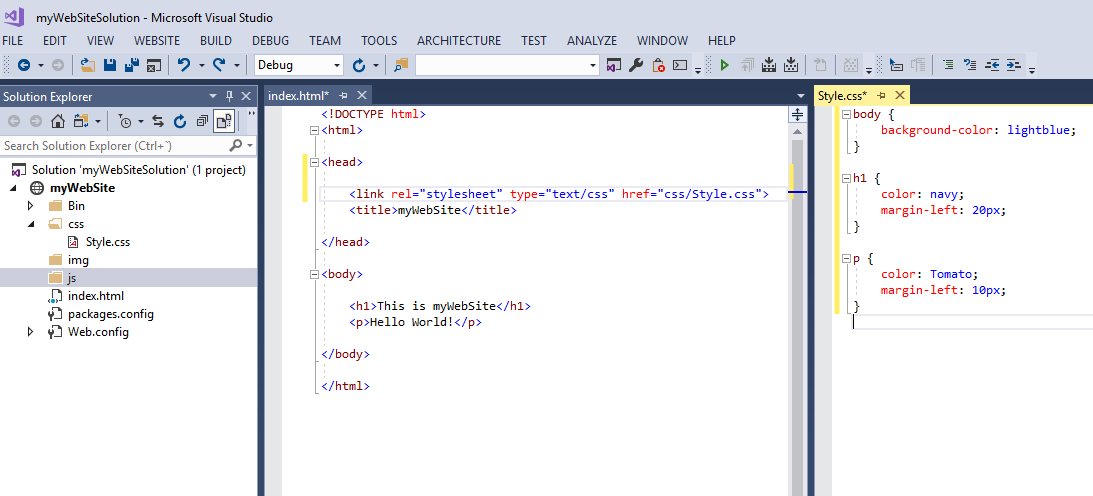
\includegraphics[width= \textwidth]{Figures/Projects/css1}
    \caption{Result of myWebSite project, main files opened and structure of the project seen in the Solution Explorer.}
    \label{fig:css1}
\end{figure}

\begin{figure}
    \centering
    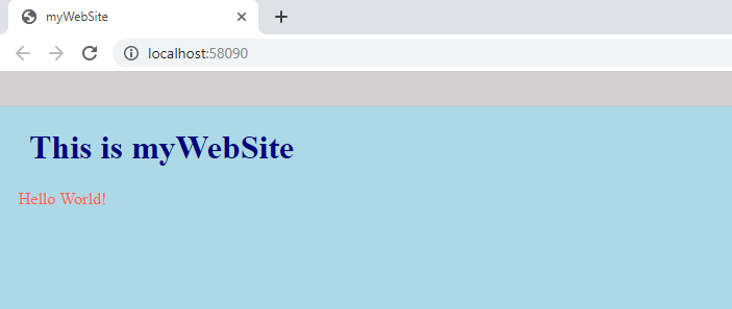
\includegraphics[width=  \textwidth]{Figures/Projects/css2}
    \caption{Result of myWebSite project after including style, using Google Chrome browser.}
    \label{fig:css2}
\end{figure}

%-----------------------------------------------------------------------------------------------------------------------------

\FloatBarrier
\textbf{The third step of this example} involves a similar process, now in order to include a JavaScript file in the project. Once again, the content is defined in a external file (it could also be written in the HTML with the tags \textless script\textgreater...\textless\textbackslash script\textgreater). Hence, include the file by clicking with the right button in the \texttt{js} folder and going to \textit{Add/Add New Item...}. There, in \textit{Installed/Visual C\#} select \textit{JavaScript File} and name it \texttt{JavaScript.js}, adding finally the file with \textit{Add} button.

Include at the end of the body of the html file the line seen in the Code \ref{lst:pro5}. It makes use of the same tags but in this case the \texttt{src }attribute tells the browser where to find the script. External scripts are practical when the same code is used in many different web pages. Notice that the style is charged at the beginning of the html file in order to have the style orders defined before the content appears. For a similar reason, the modification of the contents (js file) is not uploaded until the content is already charged in the website, and that is why the code is located at the end of the body. \vskip \baselineskip 

\begin{lstlisting}[language=HTML, caption={Line to include at the end of the HTML body in order to link the JavaScript file.}, label={lst:pro5}]
<script src="js/JavaScript.js"></script>
\end{lstlisting}

We have to write the JavaScript file and some elements to modify in the content of the webpage. In this example, we include a button with the text ``I'm a button'' written, and in the HTML file a function programmed for that button. At the same time, we include an identifier for the element to be modified when clicking in the button, let's say for example the paragraph ``Hello world!''. This identifier (HWid) is used to specify (in the function) the element that has to change. Hence, the HTML file should be changed to be like the seen in the Code \ref{lst:java1}. Notice how the button has the attribute type and the function (called in this case ``myFunction'') has the order to make when clicking (\textit{onclick}). \vskip \baselineskip

\begin{lstlisting}[basicstyle=\small, language=HTML, caption={HTML file with a new button included, an identifier in the paragraph element and the link to the \texttt{.js} file.}, label={lst:java1}]
<!DOCTYPE html>
<html>

<head>

<link rel="stylesheet" type="text/css" href="css/Style.css">
<title>myWebSite</title>

</head>

<body>

<h1>This is myWebSite</h1>
<p id="HWid">Hello World!</p>
<button type="button" onclick="myFunction()">I'm a button</button>

<script src="js/JavaScript.js"></script>

</body>

</html> 
\end{lstlisting}


\FloatBarrier
\textbf{Finally}, open in Visual Studio the file \texttt{JavaScript.js} and copy there the code seen in \ref{lst:java2} in order to define the function. When finished, press on \textit{Build} and later in \textit{Start} and Visual will show the result. It should be like the Figure \ref{fig:js1} and the webpage, after pushing the button created, should be like the Figure \ref{fig:js2}. \vskip \baselineskip 

\newpage
\begin{lstlisting}[basicstyle=\small, language=HTML, caption={\textit{myFunction} code defined in the JavaScript file, it changes the text found with the identifier ``HWid''.}, label={lst:java2}]
function myFunction() {
document.getElementById("HWid").innerHTML="Hello Universe!"
}
\end{lstlisting}

\begin{figure}
    \centering
    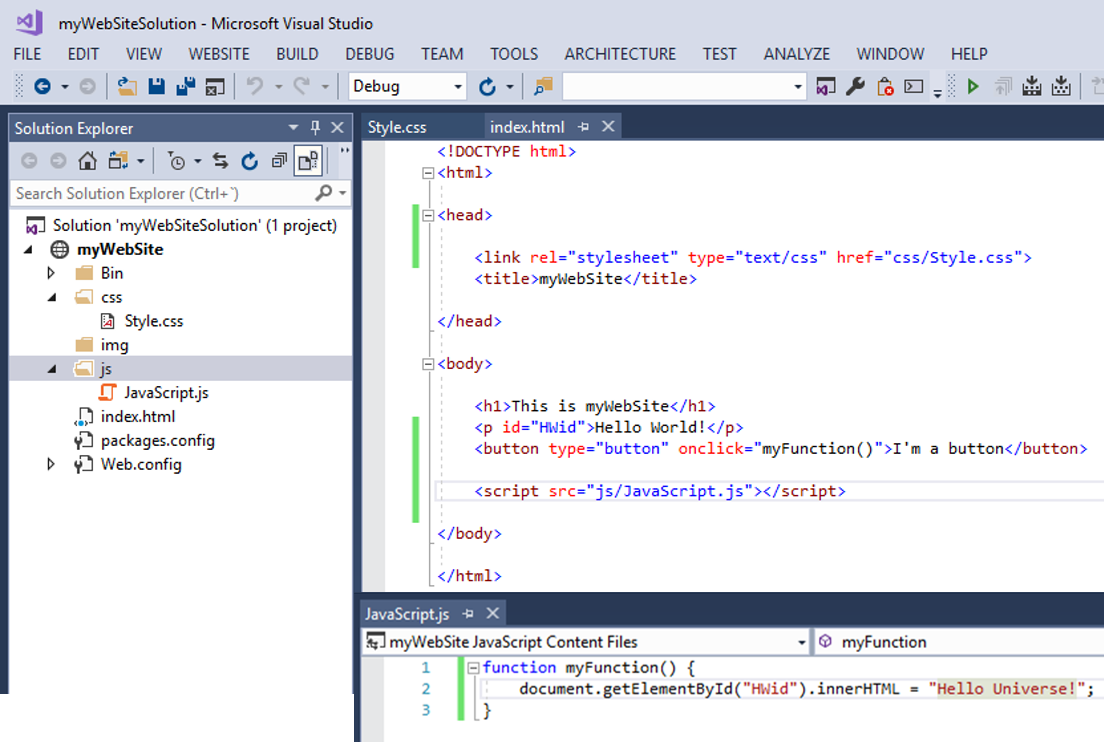
\includegraphics[width= \textwidth]{Figures/Projects/js1bis}
    \caption{Result of myWebSite project, index and script opened and the structure of the project seen in the Solution Explorer.}
    \label{fig:js1}
\end{figure}

\begin{figure}
    \centering
    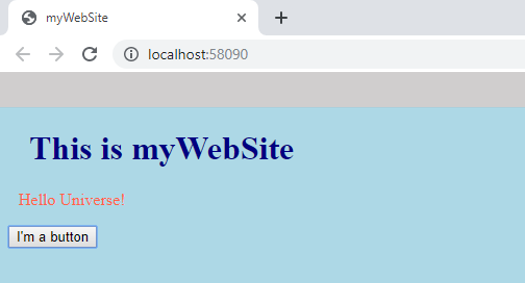
\includegraphics[width= \textwidth]{Figures/Projects/js2}
    \caption{Result of myWebSite project after including style and a script, using Google Chrome browser.}
    \label{fig:js2}
\end{figure}



    \FloatBarrier
    \section{Web Application: Fundamentals}

A website usually consists of many files: text content, code, style sheets, media content, etc. When building a website, it is necessary to assemble these files into structure on your local computer, make sure they can talk to one another, and get all the content looking right before it is uploaded to a server. A common distribution of folders and files (extracted from \url{https://developer.mozilla.org}) in a web project involves:

\begin{enumerate}[nosep]
    \item \textbf{\texttt{index.html}:} This file generally contains your homepage content (the text and images that people see when they first go to the site). Using your text editor, you can create a new file called \texttt{index.html} and save it just inside your test-site folder.
    \item \textbf{images folder:} This folder contains all the images that you use on your site.
    \item \textbf{styles folder:} This folder contains the CSS code used to style the content (for example, setting text and background colours).
    \item \textbf{scripts folder:} This folder contains all the JavaScript code used to add interactive functionality to the site (e.g. buttons that load data when clicked).    
\end{enumerate}

In conclusion, mainly three types of files contain the code necessary to create a web project: \textbf{HTML, CSS} and \textbf{JS}. The first one contains the static template of the webpage, the code that is used to structure the content and the webpage itself. Here it is decided if the webpage shows paragraphs, bullet points, images, tables, etc. and at the same time the content is linked. 

HTML (Hypertext Markup Language) is a markup language, hence, the file is constructed using a series of elements (tags are used to create the elements) that define every instruction we want to apply to an specific piece of content. For example, the enclosing tags can make a word hyperlink to somewhere else, italicize words and more. There are tags for every function or behaviour we want to define.

CSS and JS files are linked to the main HTML file using a file path so one file (main HTML file) knows where another one is. For example, the header of the \texttt{index.html} contains different routes to the style files (CSS), in addition, the body of the main HTML file also contains routes to images, videos and rest of the material that the webpage has. 

CSS (Cascading Style Sheets) is the code used to provide style to the content referred in the HTML file, this means that here we are going to decide whether the words are black or red, the decoration around the images or the aspect of the different elements mentioned in the HTML file. CSS is a \textit{style sheet language}, we can select individually elements in the main file and change the style. In addition, we can apply the same configuration to a specific group of elements that share the same aspect. 

JS makes reference to JavaScript, a programming language that adds interactivity to the website. With these files we can decide what the webpage shows when a button is pressed or define some dynamic styling. These scripts have to be applied to the main HTML file and the possibilities are huge.   

Once the different files are written in our computer and the project has been finished, all the information is uploaded to the server, a hardware and software tool that is activated at all times (in the case of a public website for example) waiting for the clients. If this server is accessible through the internet, it will be waiting for a client all over the world. When a user writes the specific IP address in its browser (or the URL assigned to our server and port), then the software part of the server will receive the request and answer. If the access is permitted, then the server will send over the internet the webpage to the computer of the client, where the browser will interpret all the information and show the website. This is a general description since there are many different ways of receiving the webpage or the web application depending on the amount of information that is processed in the client's computer or in the server. In addition, there are many protocols and applications involved in this operation. 

        \FloatBarrier
        \subsection{HTML Structure}

In this section a brief introduction to HTML is presented and some concepts related to the structure of an HTML file are treated. HTML is mainly the combination of Hypertext and Markup language. While Hypertext defines the link between the web pages, Markup language is used to define the text document and the tags that define the structure. The first version made of HTML was \textit{HTML 1.0} but the first standard version was \textit{HTML 2.0}, in 2014 HTML5 was released as a stable W3C (World Wide Web Consortium) Recommendation, meaning the specification process is complete.

HTML uses predefined tags and elements, both are read by the browser and define the properties of the content that is displayed, all the tags used have to be closed when the effect must finish. Otherwise, the property of the specific effect will continue until the end of the page. In a general case, the extent of an element is indicated by a pair of tags: the "start tag" (\textless p\textgreater) and the "end tag" (\textless /p\textgreater), an example is shown in Code \ref{lst:HTML2}. The text content of the element is placed between these tags. The start tag may also include attributes or specific routes (in the case of including images for example) within the tag. \vskip \baselineskip

\begin{lstlisting}[language=HTML, caption={Tags used in HTML with the predefined function of including paragrahps in the webpage.}, label={lst:HTML2}] 
<p> This is a paragraph. </p>
\end{lstlisting}

One of the simplest examples of HTML can be seen in the Code \ref{lst:HTML1}. It contains elements (head, title or body in this case) which are used to build the blocks of webpages, there are a lot more elements and tags that can be used for many different purposes. The first declaration (\textless !DOCTYPE html\textgreater) is used to specify the HTML version, in this case the last one, HTML5. The next tag (\textless html\textgreater) wraps all the content (is closed at the end) and is called HTML root element. Then, two main blocks are defined, the head and the body. While the head (\textless head\textgreater ... \textless /head\textgreater) contains all the HTML metadata (all the information that is not going to be visible i.e. title, page CSS, etc.), the body (\textless body\textgreater ... \textless /body\textgreater) includes all the data that the webpage has, from texts to links and everything is organized with the elements and tags mentioned (this information is visible). \vskip \baselineskip

\begin{lstlisting}[language=HTML, caption={Main structure of an HTML file.}, label={lst:HTML1}]
<!DOCTYPE html>

<html>
<head>

<title>Page Title</title>

</head>
<body>

<h1>This is a Heading</h1>
<p>This is a paragraph.</p>
<p>This is another paragraph.</p>

</body>
</html> 
\end{lstlisting}

We could write now the Code \ref{lst:HTML1} in the notepad, save it with the name \texttt{index.html} and open the file with the browser of our computer. The browser would interpret it and show the result as a common internet webpage. The browser also takes into account the HTML version written at the start of the code since not all the browser support all the versions, it must be remarked that creating webpages involves that we always depend on the browser used by the user. 


        \FloatBarrier
\newpage        
        \subsection{CSS Concepts}

CSS is a simply designed language that tries to simplify the process of making webpages presentable. It allows applying styles to webpages and enables the possibility of doing the style page independent of the HTML. When tags like \textless font\textgreater ~ and colour attributes were added to the HTML 3.2 specification, the development of large websites became complicated because fonts and colour information were added to every single page. The code became a long process. Then, W3C created CSS and the style formatting was removed from the HTML page.

The CSS syntax consist in rules that the browser interprets and then applies to the specific element in the document that is affected by the style change. In every rule-set there are a selector and a declaration block; the selector points to the specific element that is going to show the style and the declaration block contains the style. It uses the name of the property to be changed and the value, both separated by semicolons. Finally, a CSS declaration always ends with a semicolon and declaration blocks are surrounded by curly braces.

There are a lot of properties and values to apply to the design of the web, some examples are: colour, text-align, opacity, font size or font-weight. Depending on the element selected there are different options available to modify. An essential part of CSS code is the selector of the element to change, there are Selectors used to ``find'' (or select) HTML elements based on their element name, id, class, attribute, and more. The \textbf{Universal selector} simply matches the name of any element type so we will define the colour (for example) of every element in the document. On the contrary, we can choose that the property only affects to the elements with an specific \textbf{Name} like for example the paragraphs called \textless p\textgreater ... \textless /p\textgreater ~ in the example of the previous section. The \textbf{id selector} uses the id attribute of an HTML element (we can add it to the different elements used) to select a specific element. The id of the elements should be unique so we would be selecting one unique element. It uses a hash (\#) character followed by the id in order to select the element. The \textbf{class selector} selects elements with a specific class attribute (we can also add the class to the elements of our webpage). In this case it uses a (.) character, followed by the name of the class. The Code \ref{lst:CSS1} shows some examples of the notions explained. \vskip \baselineskip

\newpage
\begin{lstlisting}[language=HTML, caption={Code to include in the css file created in order to give style to the webpage.}, label={lst:CSS1}]
p {
color: red;
text-align: center;
}

#para1 {
text-align: center;
color: red;
}

.center {
text-align: center;
color: red;
}
\end{lstlisting}


        \FloatBarrier
        \subsection{JavaScript Concepts}

In the beginning, JavaScript was only used in the client side (in the browser), but node js have made possible to run also JavaScript on the server side. Today, JavaScript is everywhere (Desktop/Server/Mobile) and, as it has been said, it is used to program the behaviour of the webpages. JavaScript can change content of the HTML, change attribute values, styles, show or hide elements and more.

In the HTML file, the code of JavaScript must be written between \textless script\textgreater ~ and \textless/script\textgreater ~ tags and any number of scripts can be written in the whole document, in the body, the head, or in both. External scripts are really useful when the same code is used in different web pages and also when developing a multilayer project (all the documents are separated conceptually in different layers). In this case we reference the external file (called \texttt{ExternalScripts.js}) as it is shown in the Code \ref{lst:JS1} and the reference can be placed in the head or in the body. One of the advantages of this kind of structure is that the HTML and JavaScript files are easier to read and maintain. \vskip \baselineskip

\begin{lstlisting}[language=Java, caption={Example of the inclusion of JavaScript files in our main HTML.}, label={lst:JS1}]
<script src="ExternalScripts.js"> </script> 
\end{lstlisting}

Similar to other programming languages, a function in JavaScript is a block of code that is executed when it is called. It can be programmed that an \textit{event} (like the click in a button) calls a function and makes some changes in the webpage. \textit{Objects} in JavaScript are the most important data-type in this programming language since the whole language is formed by these blocks. The objects are similar to variables but can contain many values, each value goes together with a name (the pairs name and value are called \textit{properties}). At the same time, the objects can have \textit{methods} which are the actions that can perform. These methods are functions stored as properties. In the Code \ref{lst:JS2} (extracted from \url{https://www.w3schools.com}) an object called ``person'' is declared containing both properties and a method. Notice that the word ``this'' refers to the owner of the method, in this case the object ``person''. \vskip \baselineskip 

\begin{lstlisting}[language=Java, caption={Example of object called ``person'', declared containing both properties and a method.}, label={lst:JS2}]
var person = {
firstName: "John",
lastName : "Doe",
id       : 5566,
fullName : function() {
return this.firstName + " " + this.lastName;
}
};
\end{lstlisting}




    \FloatBarrier
    \section{Installing Node.js tools}

In order to use Node.js with Visual Studio we need the specific workload for the IDE and the JavaScript runtime environment installed in the computer. To install the workload we have to open as usually the Visual Studio Installer (as an administrator) and click on \textit{Modify}. We must select in the \textit{Workloads} (in the tab reserved for Web and Cloud) the package \textit{Node.js Development} with the predefined optional tools selected (see Figure \ref{fig:Node}). Then, we click on \textit{Modify} and wait for the process to finish the download and installation.

\begin{figure}
    \centering
    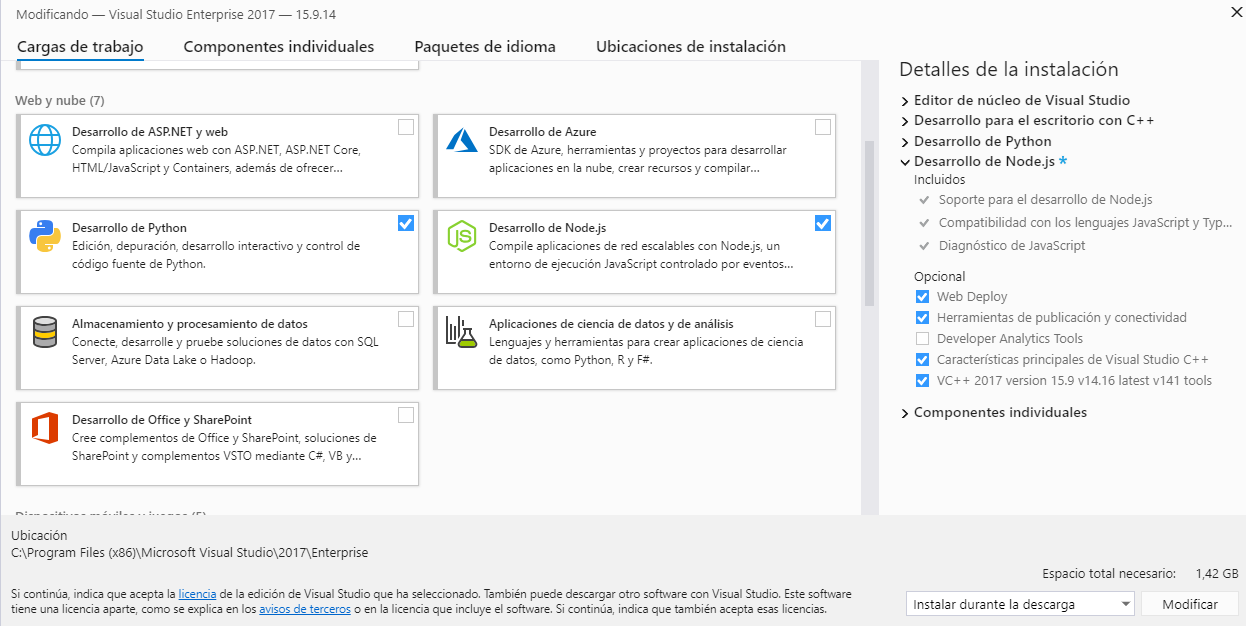
\includegraphics[width= \textwidth]{Figures/Projects/Node}
    \caption{Main window of Visual Studio Installer with the Workload to install chosen.}
    \label{fig:Node}
\end{figure}

Now, we are going to install the LTS version of the runtime (long-term support, stable release of software that is maintained by the owners for long periods of time).

\begin{enumerate}
    \item Download the installer from the Node.js website: \url{https://nodejs.org/en/download/}.
    \item Choose the \textit{recommended version for most users} installer for your computer (typically Windows 64-bit) and download the installer.
    \item Double click on the file that you have obtained.
    \item Click on \textit{Next}, accept conditions and click again on \textit{Next}.
    \item Maintain the same location for the installation and click twice in \textit{Next}.
    \item Finally, click on \textit{Install} and accept the administrator warning (Visual Studio should automatically detect the installed runtime.).
\end{enumerate}



    \FloatBarrier
    \section{Create a Node.js project}

To create a Node.js project, proceed with the following steps: 

\begin{enumerate}
    \item Open your release of Visual Studio.
    \item Click on \textit{File/New/Project...}.
    \item In the \textit{TypeScript} menu of the \textit{Installed} tab select \textit{Node.js} and then click on \textit{Blank Node.js Console Application}.
    \item Choose a name for the project. 
    \item Change the \textit{Location} of the solution, the directory will be created there.
    \item Choose the name of the solution, it does not have to be the same as the one of the project.  
    \item Select option \textit{Create directory for solution}.
    \item Click on \textit{OK}.
\end{enumerate}




    \FloatBarrier
    \section{Execute the ``Hello world'' example (Node.js)} 
    
You can check in the solution directory chosen that a folder with the project has been created, inside, the project is represented by a \texttt{.njsproj} file. In the solution explorer you will find a npm node which shows the already installed npm packages (NPM is a package manager for Node.js with thousands of free packages (or modules) to download and use).

In order to check that everything is correctly installed we run the ``Hello world" example. This example is written automatically when we select this kind of project so you can open the file \texttt{app.ts} (double-clicking on this name in the solution explorer) and check that is written something similar to the code \ref{lst:Node1}. \vskip \baselineskip

\begin{lstlisting}[language=Java, caption={``Hello world'' example written in a Node.js project.}, label={lst:Node1}]
console.log('Hello world');
\end{lstlisting}

\newpage
After building and starting the project this program opens the console and shows "Hello World" written. Follow the next steps:

\begin{enumerate}
    \item Click on \textit{BUILD + ``Name of the project''} or click on the corresponding icon.
    \item Click on \textit{DEBUG/Start Without Debugging} or click the corresponding icon.
\end{enumerate}

\begin{IN}
    If the console is immediately closed after printing ``Hello world'' in your computer, you have to force the process to wait after finishing the execution. Click on \textit{DEBUG/Options...} and look for ``NodeJS Tools", there tick the box \textit{Wait for input when process exits normally}.
\end{IN} 




    \section{Debugging a web page}
     
Generally, the main file of a web page needs to be opened by a server. Node.js allows to run a local server very easily. Hence, in order to debug a web page before it is hosted in a special server, the following steps can be accomplished:

\begin{enumerate}[nosep] 
	\item Install \verb|node.js|. 
	\item Install a http server by the following command:
	
	      \verb|>npm install http-server -g|
	      
	\item Execute the commnad: 
    
      \verb|>http-server|
      
	\item  In chrome browser type:
    
     \verb|//http://localhost:8080/index.html|
     
      and press F12. 
\end{enumerate} 

The last command will start up a http server in the local-host. 
    


    \FloatBarrier
    \section{Cordova project}

Cordova allows us to create Phone Apps starting with our previously created Web project. In order to obtain the essential tools for creating Cordova projects with Visual Studio follow these steps:

\begin{enumerate}
    \item Open Visual Studio installer as an administrator and click on \textit{Modify}.
    \item Select in the \textit{Workloads} (in the tab reserved for smartphones and games) the tools related to \textit{Development for Mobile Phones Devices with JavaScript} with the predefined optional installations selected (GIT for Windows is not needed) (see Figure \ref{fig:cor1}).
    \item In this case we also need from the \textit{Individual Components} tab the \textit{Google Android Emulator (API level 27)} and the \textit{Installation of Android SDK (API level 27)} (Figures \ref{fig:cor2} and \ref{fig:cor3}).
    \item Click on \textit{Modify} and wait for the process to finish downloading and installing.
\end{enumerate}

\begin{IN}
    This process has been tested with Visual Studio 2017, in the newer versions of the IDE we do not know if Microsoft will continue offering the Cordova tools.
\end{IN}

\begin{figure}
    \centering
    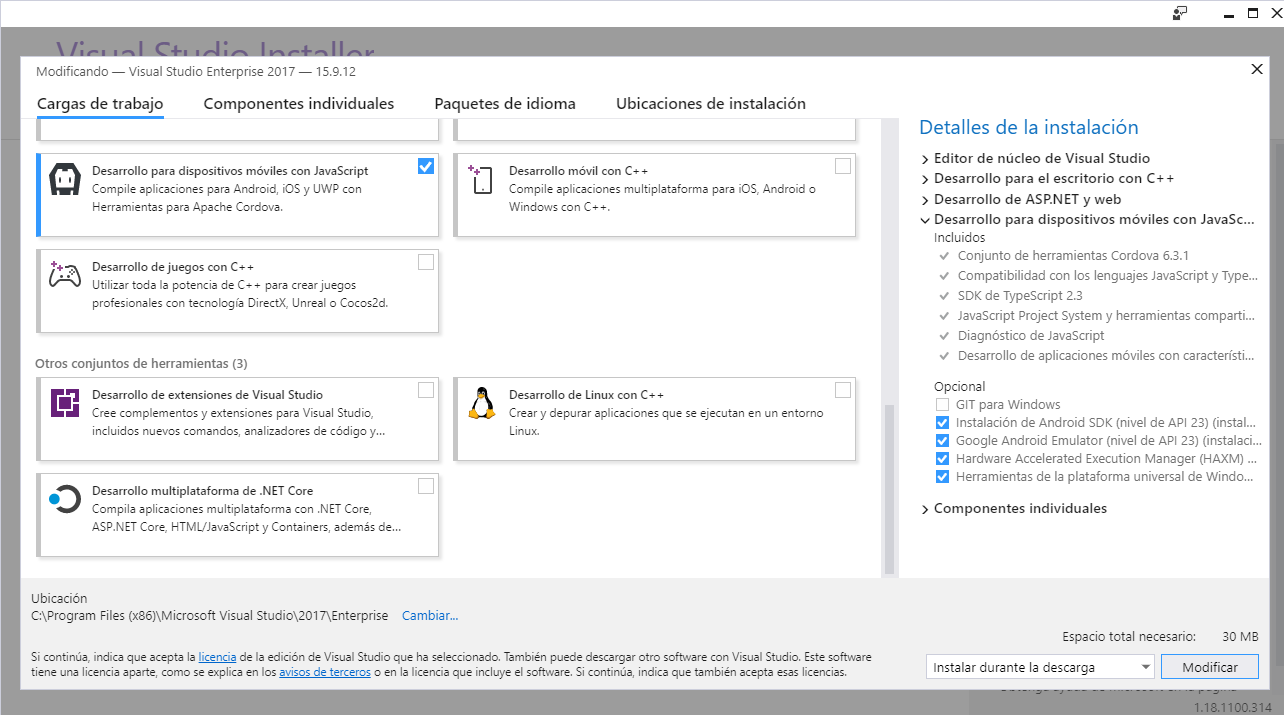
\includegraphics[width= \textwidth]{Figures/Projects/cor1}
    \caption{Main window of Visual Studio Installer with the Workload to install chosen, it installs Cordova programming tools.}
    \label{fig:cor1}
\end{figure}

\begin{figure}
    \centering
    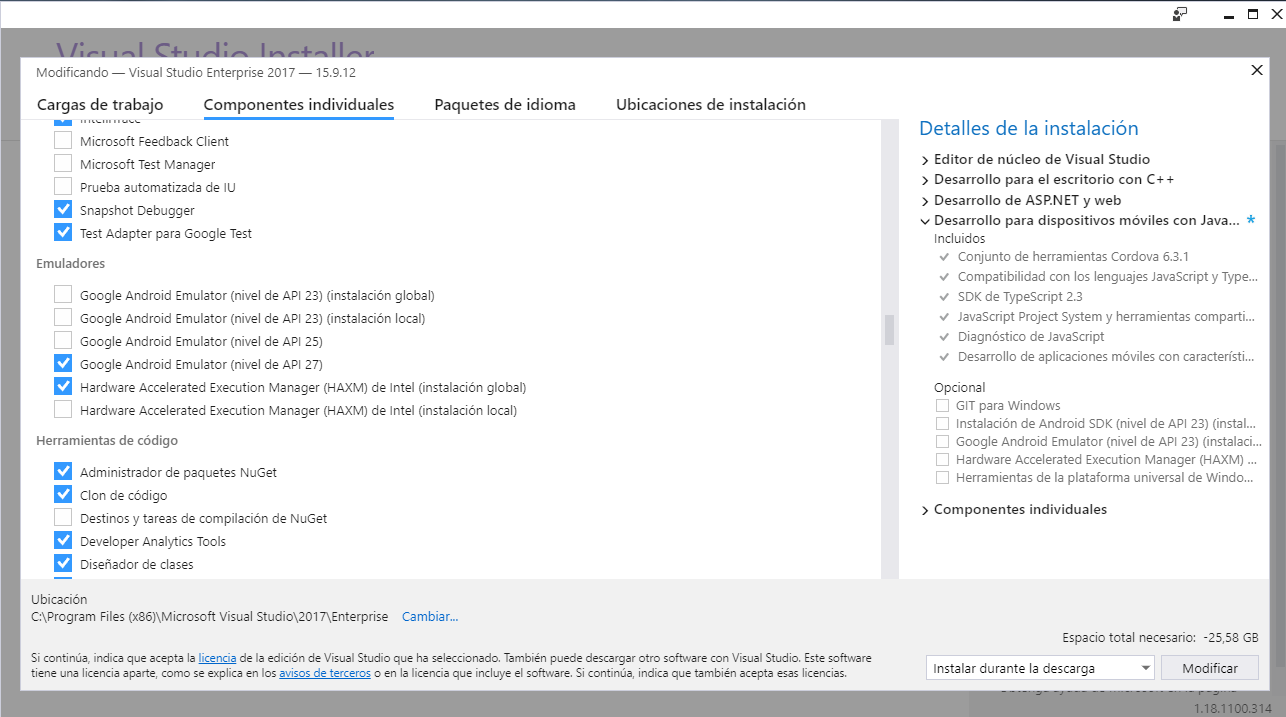
\includegraphics[width= \textwidth]{Figures/Projects/cor2}
    \caption{Main window of Visual Studio Installer with the Individual Components to install chosen. The right version for Android applications is selected.}
    \label{fig:cor2}
\end{figure}

\begin{figure}
    \centering
    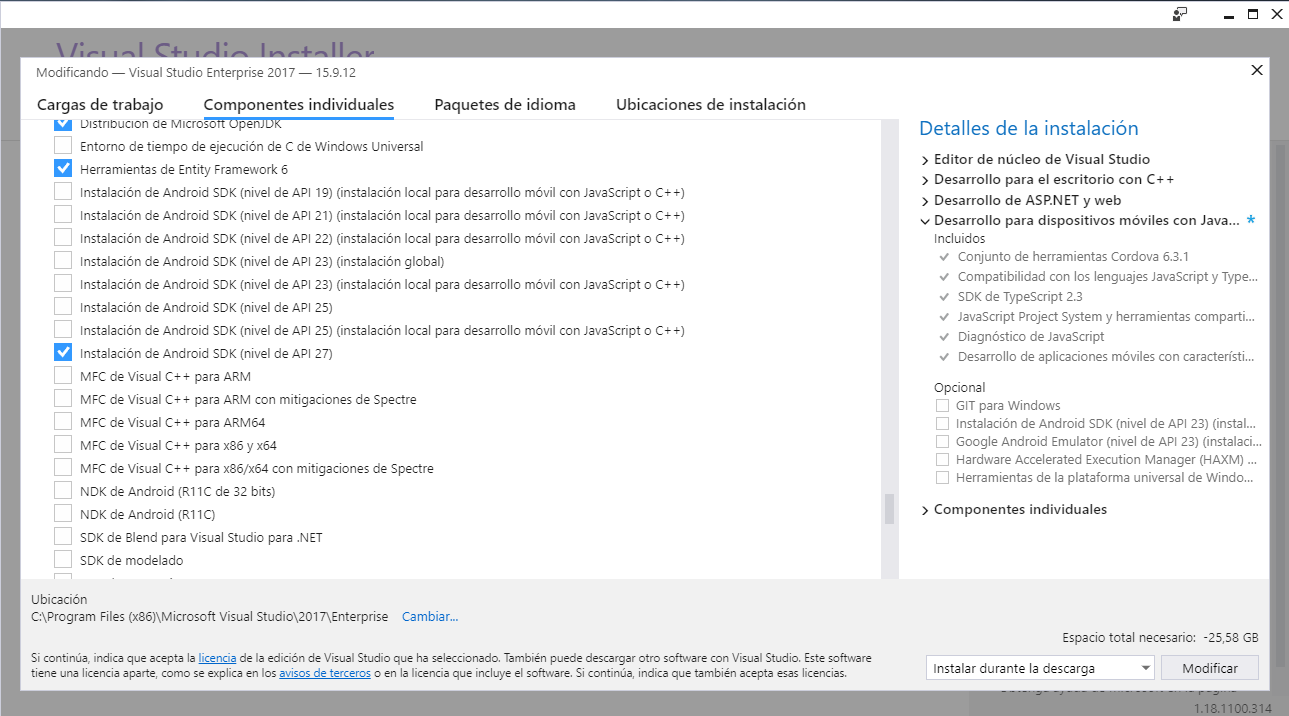
\includegraphics[width= \textwidth]{Figures/Projects/cor3}
    \caption{Main window of Visual Studio Installer with more Individual Components to install in order to obtain Cordova programming tools. The right version for Android applications is selected.}
    \label{fig:cor3}
\end{figure}


\FloatBarrier
The next step is to create a project with Cordova, follow these steps:

\begin{enumerate}
    \item Click on \textit{File/New/Project...} or press Ctrl+Shift+N (Figure \ref{fig:Cordova1}).
    \item Choose \textit{Blank App (Apache Cordova)} in the tab \textit{Installed/JavaScript/Mobile Apps}. Name the project ``HelloWorld'' (this will be the name of the app), choose the location of the project and name the solution: ``CordovaProjects'' for example (Figure \ref{fig:Cordova2}).
    \item Click on \textit{OK}.
    \item The aspect by default of the solution and project is seen in Figure \ref{fig:Cordova3}.
\end{enumerate}


\newpage
Now we can simulate and execute the HelloWorld example starting with the webpage created in the previous section:

\begin{enumerate}
    \item Select all the files inside the \texttt{www} folder and delete them.
    \item Click with the right button of your mouse on the folder \texttt{www} and click on \textit{Add/Existing Item...}, navigate to the location of the files created in the section \ref{sec:Web} (HTML/CSS/JS) and add to the project all the files and folders. The final aspect of the project opened is shown in the Figure \ref{fig:Cordova4}.
    \item Deploy the menu with the solution configurations (Debug is shown by default) and open the Configuration Manager.
    \item In order to simulate the result of our App, deselect \textit{Deploy} when the Configuration \textit{Debug} and Platform \textit{Android} are selected (Figure \ref{fig:Cordova5}).
    \item Close the Configuration Manager and check that the configuration of the solution is marked as \textbf{Debug - Android - Simulate in Browser LG G5}. Click on the execution button and the result will appear in your default browser (Chrome, Firefox, etc. Figure \ref{fig:Cordova6}).
    \item If the results of the simulation are correct, the .apk file can be generated in order to install the App in your Android phone.
    \item In the same place where the simulation is chosen, now choose \textit{Device} (Figure \ref{fig:Cordova7}). Execute the project and a \texttt{.apk} file will appear in the folder of the project, in the path 
    
    \textit{platforms\textbackslash android\textbackslash build\textbackslash outputs\textbackslash apk}.
    
    \item Transfer that file to your smartphone and execute it (Figure \ref{fig:CordovaApp}).
\end{enumerate}

\begin{IN}
    When building and executing the project, the first time, an error like the next one could appear:\newline
    
    \textit{Error: Failed to run ``javac -version'', make sure that you have a JDK installed.} \newline
    \textit{You can get it from: http://www.oracle.com/technetwork/java/javase /downloads.} \newline 
    
    If it is your case, install or update the JDK (Java Development Kit) of Java. We have fixed this problem by installing not only the release 12.0.2 of the JDK but also installing the update 8u221 for the previous release of the JDK (Java SE 8). \newline
    
    In order to install those complements open the website and go through the page looking for the Download button of the Oracle JDK of the version \textit{Java SE 12.0.2} and the JDK of \textit{Java SE 8u221}. Click first on one button and download and install the file \texttt{jdk-12.0.2\_windows-x64\_bin.zip}. Later, click on the second one and download and install \texttt{jdk-8u221-windows-x64.exe}.
\end{IN}

\begin{figure}
    \centering
    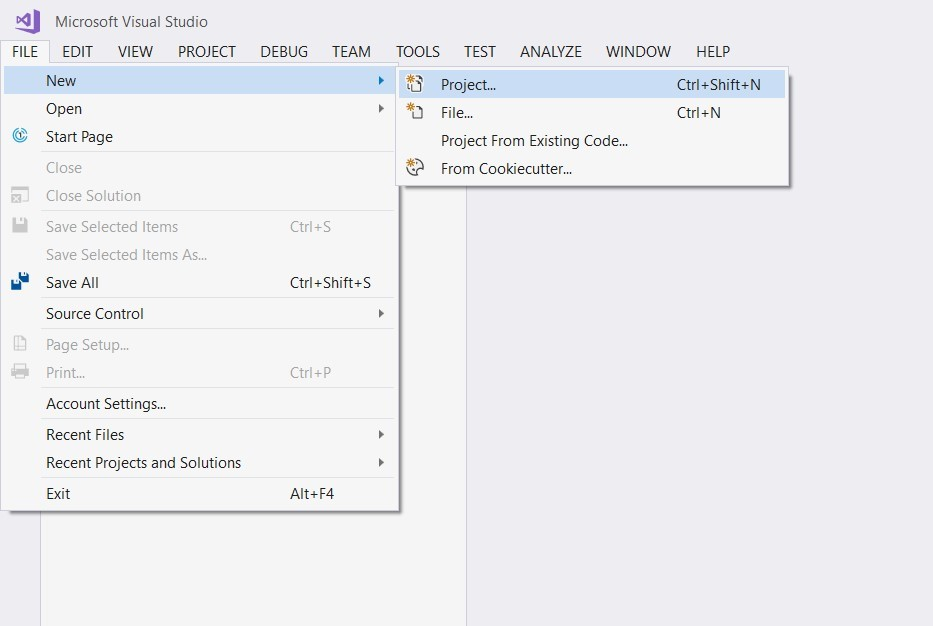
\includegraphics[width=0.9 \textwidth]{Figures/Cordova1}
    \caption{First step in order to crate a Cordova project.}
    \label{fig:Cordova1}
\end{figure}

\begin{figure}
    \centering
    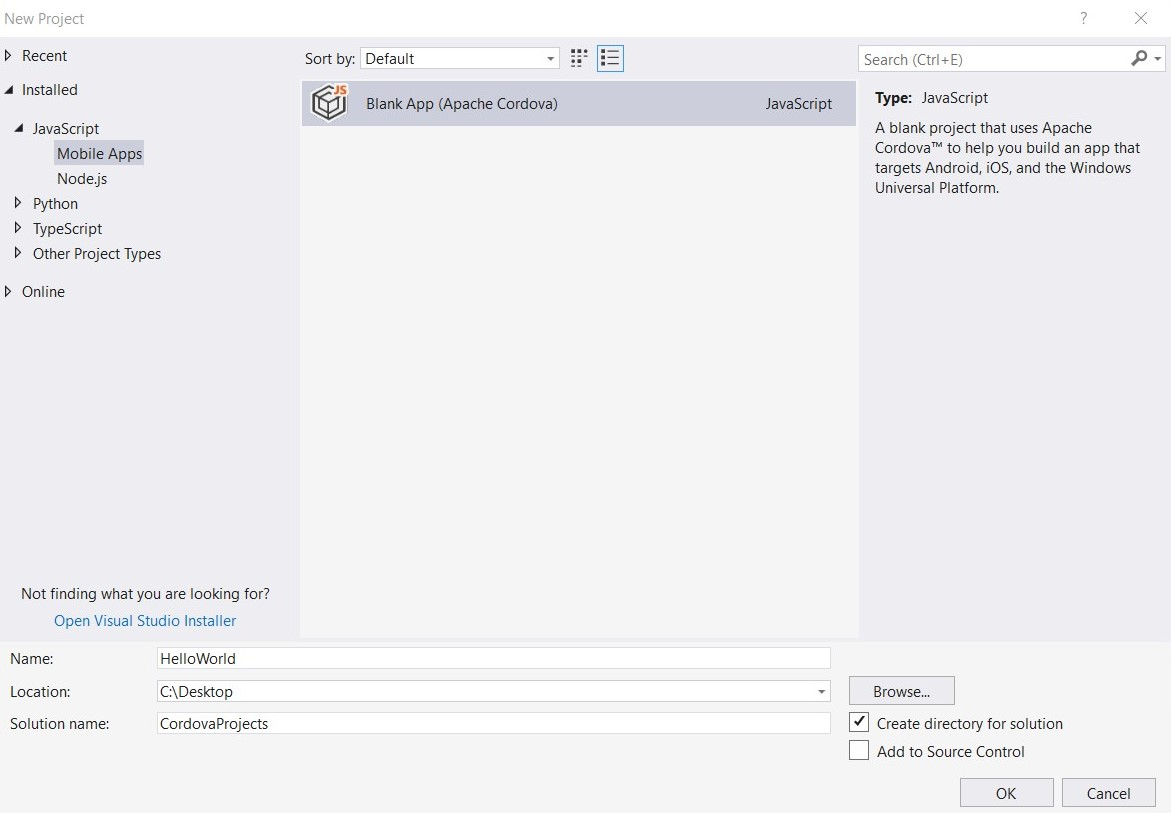
\includegraphics[width= 0.9 \textwidth]{Figures/Cordova2}
    \caption{Empty Cordova project, do not forget to choose a Name for the project (name of the app), a Solution Name and the location to store the folders and files.}
    \label{fig:Cordova2}
\end{figure}

\begin{figure}
    \centering
    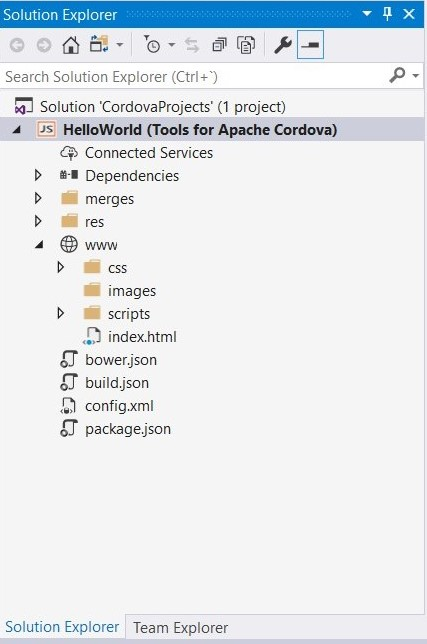
\includegraphics[width= 0.6 \textwidth]{Figures/Cordova3}
    \caption{Initial aspect of the project, the folder \texttt{www }is where all the files of the HTML/CSS/JS project will be stored.}
    \label{fig:Cordova3}
\end{figure}

\begin{figure}
    \centering
    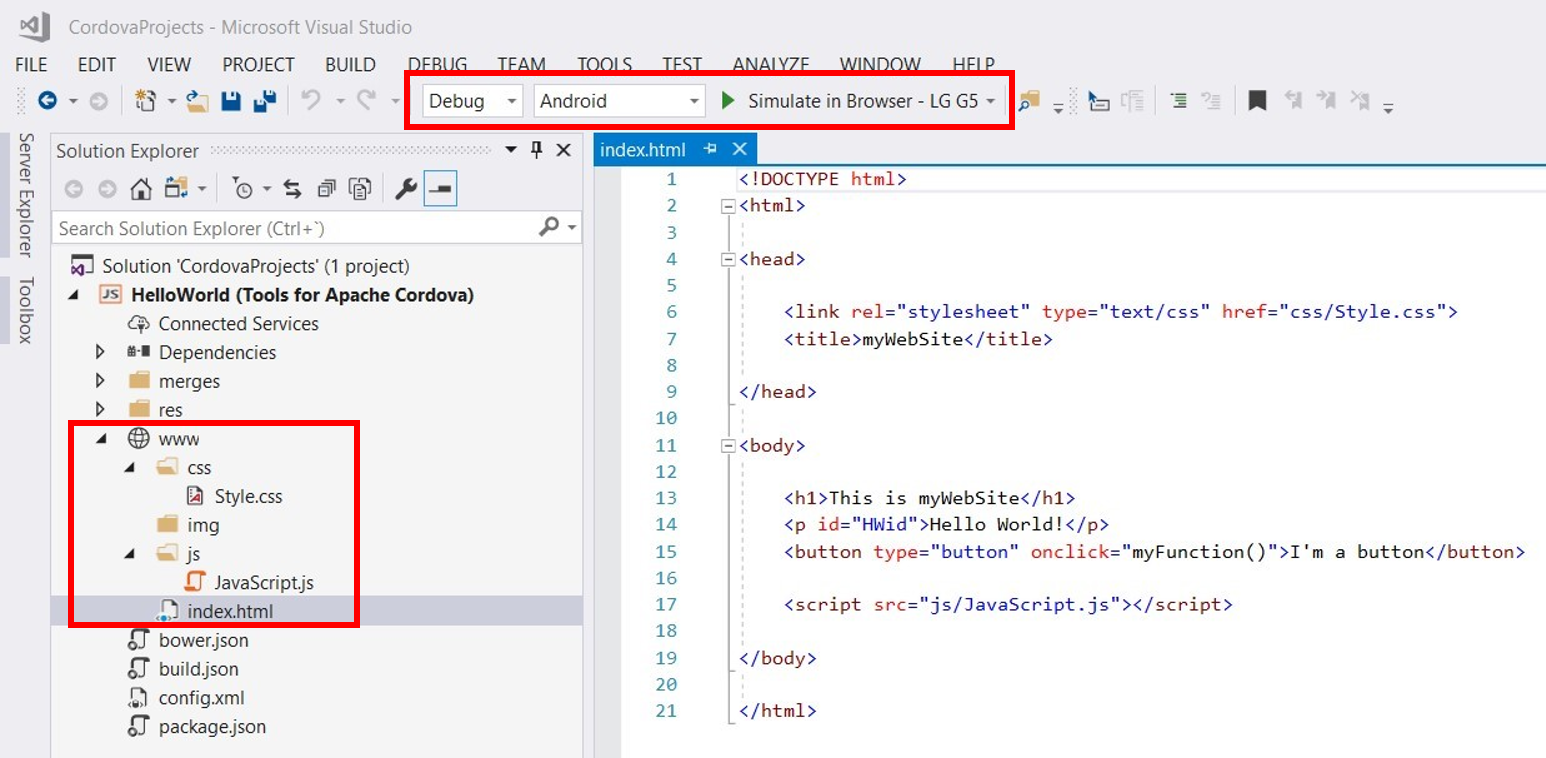
\includegraphics[width= \textwidth]{Figures/Cordova4}
    \caption{Solution explorer with our files already included, the \texttt{index.html} that we created in the previous sections is displayed.}
    \label{fig:Cordova4}
\end{figure}

\begin{figure}
    \centering
    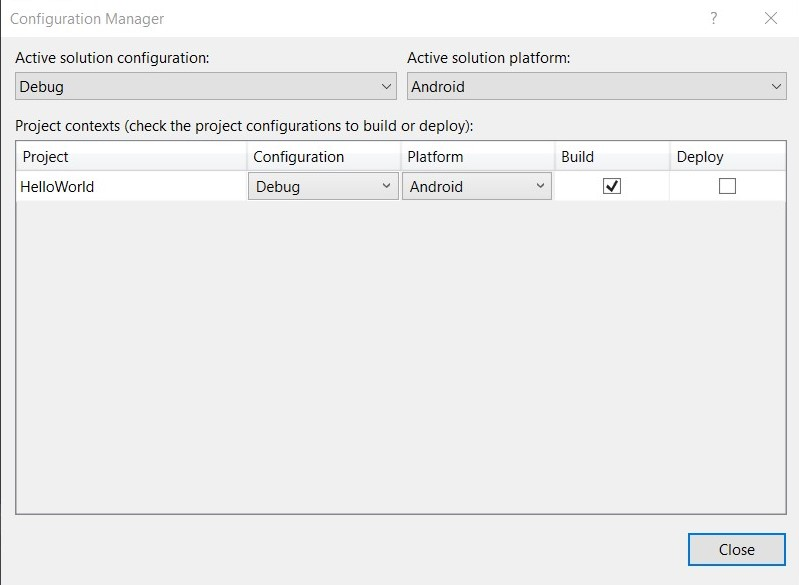
\includegraphics[width=0.8 \textwidth]{Figures/Cordova5}
    \caption{Configuration Manager of the solution, here we deselect the Deploy option that allows to transfer the \texttt{.apk} file to the smartphone automatically when it is connected.}
    \label{fig:Cordova5}
\end{figure}

\begin{figure}
    \centering
    
\includegraphics[width= 0.6\textwidth]{Figures/Cordova6}
    \caption{Simulation of the App in the browser, in this case simulating a LG G5 smartphone. The result has the same aspect ratio as the smartphone screen.}
    \label{fig:Cordova6}
\end{figure}

\begin{figure}
    \centering
    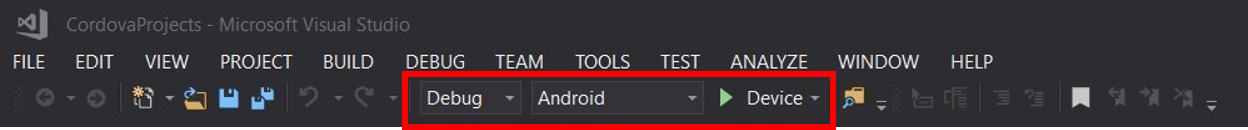
\includegraphics[width= \textwidth]{Figures/Cordova7}
    \caption{Configuration to choose in order to generate the \texttt{.apk} file that will be installed in the Android smartphone.}
    \label{fig:Cordova7}
\end{figure}

\begin{figure}
    \centering
    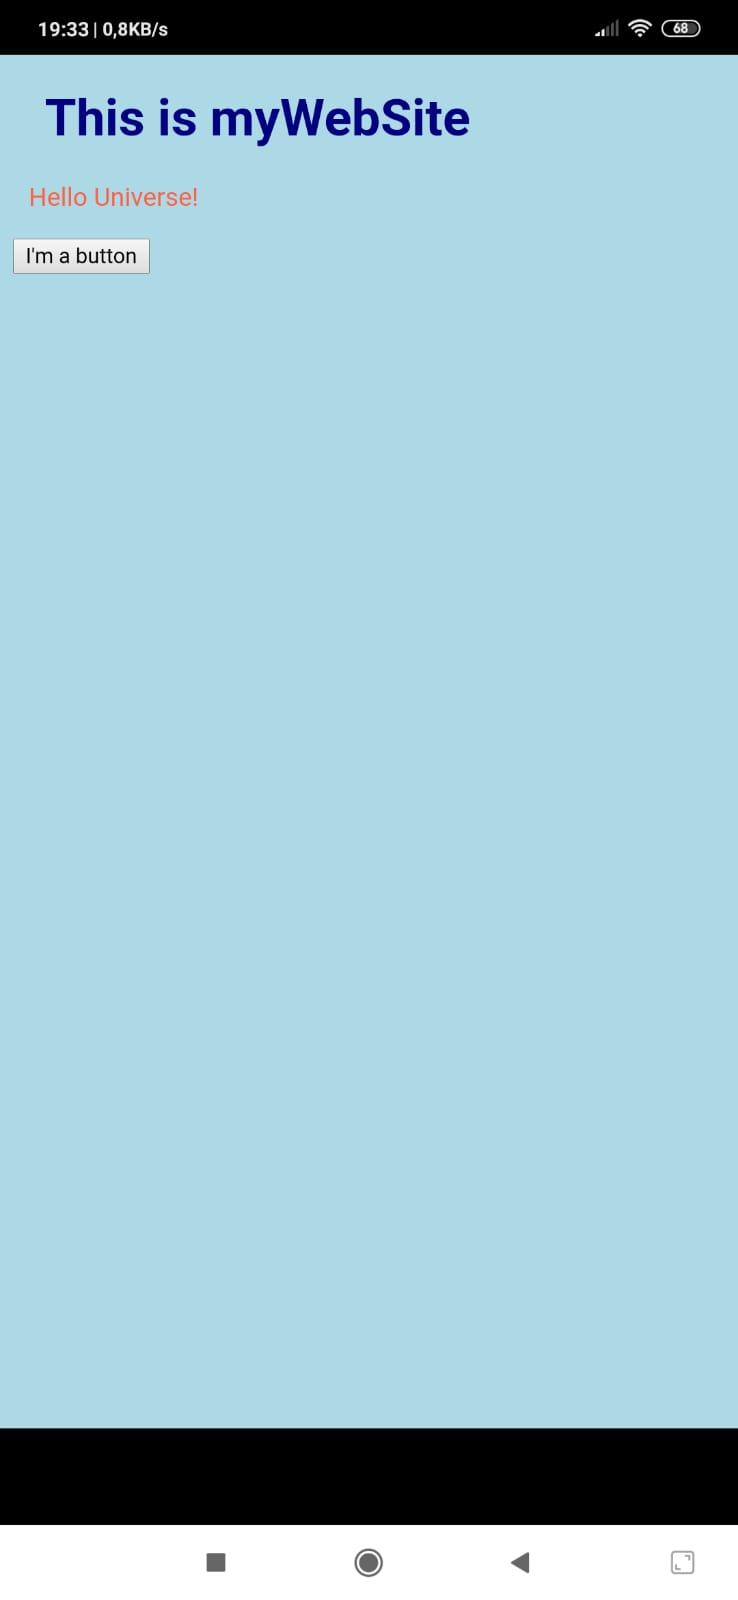
\includegraphics[width= 0.6 \textwidth]{Figures/CordovaApp}
    \caption{Phone Application installed in the smartphone through the \texttt{.apk} file.}
    \label{fig:CordovaApp}
\end{figure}



















 